\documentclass[12pt, a4paper, oneside]{article}
\usepackage{graphicx}
\usepackage{arial}
\renewcommand{\familydefault}{\sfdefault}
\usepackage[T1]{fontenc}
\usepackage[polish]{babel}
\usepackage[utf8]{inputenc}
\usepackage{lmodern}
\usepackage[left=2cm,right=2cm,top=2cm,bottom=2cm]{geometry}
\selectlanguage{polish}
\usepackage{booktabs, multicol, multirow}
\usepackage{longtable}

\begin{document}
\section{Wykorzystane wzory}
Niepewność pomiaru napięcia miernikiem Metex M-4630:
\begin{equation}
u(U)=0.05\%~rdg + 3\cdot dgt
\end{equation}
Wyznaczanie parametru $\Delta U_2$:
\begin{equation}
\Delta U_2=|U_{2_i} - U_{2_{i+1}}|,
\end{equation}
\indent gdzie: $U_{2_i}$ jest argumentem, dla którego funkcja $I_a(U_2)$ osiąga lokalne maksimum\\

\noindent Niepewność wyznaczonego parametru $\Delta U_2$:
\begin{equation}
u_C(\Delta U_2)=\sqrt{(\frac{\partial \Delta U_2}{\partial U_{2_i}})^2\cdot u^2(U_{2_{i}}) + (\frac{\partial \Delta U_2}{\partial U_{2_{i+1}}})^2\cdot u^2(U_{2_{i+1}})}=\sqrt{u^2(U_{2_{i}})+u^2(U_{2_{i+1}})}
\end{equation}
Energia wzbudzenia atomu:
\begin{equation}
E=e\cdot\Delta U_2
\end{equation}
Niepewność wyznaczonej energii wzbudzenia atomu:
\begin{equation}
u_C(E)=|\frac{\partial E}{\partial \Delta U_2}\cdot u_C(\Delta U_2)|=e \cdot u_C(\Delta U_2)
\end{equation}
Długość fali fotonu emitowanego przy przejściu atomu ze stanu zbudzonego do podstawowego:
\begin{equation}
\lambda = \frac{h\cdot c}{E}
\end{equation}
Niepewność wyznaczonej długości fali emitowanego fotonu:
\begin{equation}
u_C(\lambda)= |\frac{\partial \lambda}{\partial E}\cdot u_C(E)|=\frac{h\cdot c}{E^2}\cdot u_C(E)
\end{equation}
\section{Przykładowe obliczenia}
Niepewność pomiaru napięcia miernikiem Metex M-4630:
\begin{center}
$u(25.15)=0.05\%\cdot25.15 + 3\cdot 0.01=0.042575=0.043~[V]$
\end{center}
Wyznaczanie parametru $\Delta U_2$:
\begin{center}
$\Delta U_2=|19.03 - 36.04| = 17.01~[V]$
\end{center}
Niepewność wyznaczonego parametru $\Delta U_2$:
\begin{center}
$u_C(37.97)=\sqrt{(0.04)^2+(0.049)^2}=\sqrt{0.0016 + 0.002401}= 0.063253=0.064~[V]$
\end{center}
Energia wzbudzenia atomu:
\begin{center}
$E=1\cdot 17.01=17.01~[eV]$
\end{center}
Niepewność wyznaczonej energii wzbudzenia atomu:
\begin{center}
$u_C(17.01)=1\cdot 0.064=0.064~[eV]$
\end{center}
Długość fali fotonu emitowanego przy przejściu atomu ze stanu zbudzonego do podstawowego:
\begin{center}
$\lambda = \frac{4.13\cdot 10^{-15} \cdot 3 \cdot 10^8}{17.01}=7.2839\cdot10^{-8}=72.839~[nm]$
\end{center}
Niepewność wyznaczonej długości fali emitowanego fotonu:
\begin{center}
$u_C(7.2839\cdot10^{-8})=\frac{4.13\cdot10^{-15}\cdot 3\cdot10^8}{(17.01)^2}\cdot 0.064=0,00274\cdot10^{-7}=2.8\cdot10^{-10}=0.28~[nm]$
\end{center}
\clearpage
\section{Wyniki pomiarów i opracowanie}
% Table generated by Excel2LaTeX from sheet 'Arkusz1'
\begin{longtable}{|c|c|c|c|}
\caption{Wyniki pomiarów napięcia przyspieszającego, odpowiadającego mu prądu anodowego oraz niepewności pomiarowe}
\label{variability_impl_mech}
\endfirsthead
\endhead
\hline
    $U_2~[V]$ & $u(U_2)~[V]$ & $I_a~[nA]$ & $u(I_a)~[nA]$ \\\hline
    0.00 & 0.03 & 3.625 & 0.032 \\\hline
    1.010 & 0.031 & 3.626 & 0.032 \\\hline
    2.000 & 0.031 & 3.628 & 0.032 \\\hline
    3.000 & 0.032 & 3.645 & 0.032 \\\hline
    4.000 & 0.032 & 3.615 & 0.032 \\\hline
    5.000 & 0.033 & 3.675 & 0.032 \\\hline
    6.000 & 0.033 & 3.676 & 0.032 \\\hline
    7.000 & 0.034 & 3.680 & 0.032 \\\hline
    8.000 & 0.034 & 3.700 & 0.032 \\\hline
    9.040 & 0.035 & 3.701 & 0.032 \\\hline
    10.080 & 0.036 & 3.712 & 0.032 \\\hline
    11.060 & 0.036 & 3.716 & 0.032 \\\hline
    12.000 & 0.036 & 3.719 & 0.032 \\\hline
    13.190 & 0.037 & 3.725 & 0.032 \\\hline
    14.190 & 0.038 & 3.729 & 0.032 \\\hline
    15.040 & 0.038 & 3.763 & 0.032 \\\hline
    16.130 & 0.039 & 3.807 & 0.032 \\\hline
    16.990 & 0.039 & 3.813 & 0.032 \\\hline
    18.10 & 0.04 & 3.827 & 0.032 \\\hline
    19.03 & 0.04 & 3.833 & 0.032 \\\hline
    20.080 & 0.041 & 3.825 & 0.032 \\\hline
    20.960 & 0.041 & 3.824 & 0.032 \\\hline
    21.980 & 0.041 & 3.814 & 0.032 \\\hline
    23.190 & 0.042 & 3.803 & 0.032 \\\hline
    24.180 & 0.043 & 3.792 & 0.032 \\\hline
    25.150 & 0.043 & 3.849 & 0.032 \\\hline
    25.900 & 0.043 & 3.876 & 0.032 \\\hline
    27.170 & 0.044 & 3.932 & 0.032 \\\hline
    28.070 & 0.045 & 3.990 & 0.032 \\\hline
    29.070 & 0.045 & 4.035 & 0.033 \\\hline
    30.020 & 0.046 & 4.224 & 0.033 \\\hline
    31.020 & 0.046 & 4.369 & 0.033 \\\hline
    31.960 & 0.046 & 4.386 & 0.033 \\\hline
    32.900 & 0.047 & 4.401 & 0.033 \\\hline
    33.910 & 0.047 & 4.521 & 0.033 \\\hline
    34.940 & 0.048 & 4.643 & 0.033 \\\hline
    36.040 & 0.049 & 4.752 & 0.033 \\\hline
    37.160 & 0.049 & 4.602 & 0.033 \\\hline
    38.03 & 0.05 & 4.629 & 0.033 \\\hline
    38.94 & 0.05 & 4.562 & 0.033 \\\hline
    40.070 & 0.051 & 4.495 & 0.033 \\\hline
    40.890 & 0.051 & 4.404 & 0.033 \\\hline
    $U_2~[V]$ & $u(U_2)~[V]$ & $I_a~[nA]$ & $u(I_a)~[nA]$ \\\hline    
    42.100 & 0.052 & 4.265 & 0.033 \\\hline
    43.110 & 0.052 & 4.172 & 0.033 \\\hline
    43.940 & 0.052 & 4.183 & 0.033 \\\hline
    44.970 & 0.053 & 4.235 & 0.033 \\\hline
    46.130 & 0.054 & 4.350 & 0.033 \\\hline
    46.970 & 0.054 & 4.483 & 0.033 \\\hline
    48.110 & 0.055 & 4.651 & 0.033 \\\hline
    49.110 & 0.055 & 4.839 & 0.033 \\\hline
    50.010 & 0.056 & 4.987 & 0.033 \\\hline
    51.020 & 0.056 & 5.252 & 0.033 \\\hline
    52.090 & 0.057 & 5.506 & 0.033 \\\hline
    53.030 & 0.057 & 5.723 & 0.033 \\\hline
    54.000 & 0.057 & 5.881 & 0.033 \\\hline
    54.910 & 0.058 & 6.004 & 0.034 \\\hline
    56.000 & 0.058 & 6.085 & 0.034 \\\hline
    57.000 & 0.059 & 6.132 & 0.034 \\\hline
    57.980 & 0.059 & 6.056 & 0.034 \\\hline
    58.98 & 0.06 & 6.043 & 0.034 \\\hline
    59.91 & 0.06 & 5.884 & 0.033 \\\hline
    61.040 & 0.061 & 5.758 & 0.033 \\\hline
    61.850 & 0.061 & 5.695 & 0.033 \\\hline
    62.860 & 0.062 & 5.669 & 0.033 \\\hline
    64.010 & 0.063 & 5.682 & 0.033 \\\hline
    64.910 & 0.063 & 5.703 & 0.033 \\\hline
    65.960 & 0.063 & 5.793 & 0.033 \\\hline
    67.000 & 0.064 & 5.924 & 0.033 \\\hline
    68.050 & 0.065 & 6.138 & 0.034 \\\hline
    69.170 & 0.065 & 6.413 & 0.034 \\\hline
    70.060 & 0.066 & 6.651 & 0.034 \\\hline
    71.070 & 0.066 & 6.954 & 0.034 \\\hline
    71.950 & 0.066 & 7.238 & 0.034 \\\hline
    73.080 & 0.067 & 7.590 & 0.034 \\\hline
    74.050 & 0.068 & 8.129 & 0.035 \\\hline
    75.050 & 0.068 & 8.722 & 0.035 \\\hline
    75.960 & 0.068 & 9.195 & 0.035 \\\hline
    77.010 & 0.069 & 9.618 & 0.035 \\\hline
    77.870 & 0.069 & 9.987 & 0.035 \\\hline
    78.74 & 0.07 & 10.370 & 0.036 \\\hline
    79.52 & 0.07 & 10.717 & 0.036 \\\hline
\end{longtable}%
\clearpage
\begin{figure}[h]
\centering
\caption{Wykres zależności prądu anodowego od napięcia przyspieszającego}
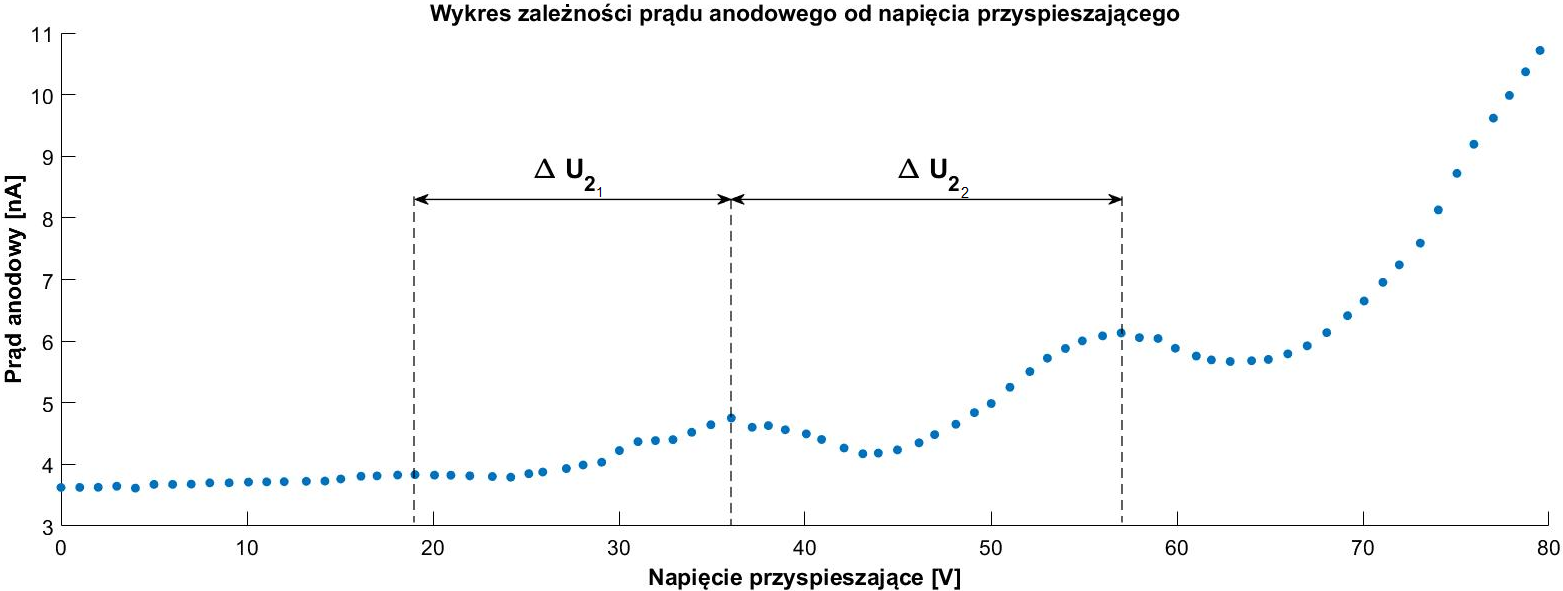
\includegraphics[width=17.5cm,height=7.5cm]{chart1.png}
\end{figure}
Z wykresu można wnioskować, że funkcja posiada 3 maksima, kolejno dla wartości $U_2$: 19.03, 36.04, 57. Na tej podstawie zostały wyznaczone wartości nazwane $\Delta U_{2_1}$ = (17.01 $\pm$ 0.064) V oraz $\Delta U_{2_1}$ = (20.96 $\pm$ 0.077) V.\\
\indent Jak widać wartości nie są zbieżne, a z teorii wynika, że $\Delta U_{2_1}$ = $\Delta U_{2_2}$. Z tego powodu wyznaczona zostaje wartość średnia $\bar{\Delta U_2}$ = (19.0 $\pm$ 0.2) V.\\
\indent Na podstawie $\bar{\Delta U_2}$ obliczona zostaje energia wzbudzenia atomu E = (19 $\pm$ 0.2) eV, która pozwala określić długość fali wyemitowanego fotonu $\lambda$ = (65.21 $pm$ 0.69) nm.
\section{Wnioski}
\begin{itemize}
\item W doświadczeniu, zgodnie z opisem zasilacza przyjęto, że $I_A$ $\approx$ $U_A$.
\item W okolicach drugiego maksimum na wykresie zaobserwowano pewne zaburzenia, które mogą mieć wpływ na wartości pomiaru, jednak trudno jest je oszacować.
\item Wyniki otrzymano przy napięciach $U_1$ = 1.53 V oraz $U_3$ = 8.53 V
\item Wartości szczytowe prądu to:
\begin{itemize}
\item (3.833 $\pm$ 0.032) nA przy napięciu (19.03 $\pm$ 0.04) V,
\item (4.752 $\pm$ 0.033) nA przy napięciu (36.040 $\pm$ 0.049) V,
\item (6.132 $\pm$ 0.034) nA przy napięciu (57.000 $\pm$ 0.059) V.
\end{itemize}
\item $\bar{\Delta U_2}$ = (19.0 $\pm$ 0.2) V.
\item Energia wzbudzenia atomu neonu E = (19 $\pm$ 0.2) eV
\item Długość fali fotonu emitowanego przy przejściu atomu neonu ze stanu wzbudzonego do stanu podstawowego $\lambda$ = (65.21 $\pm$ 0.69) nm - fala z dalekiego ultrafioletu, niewidoczna dla oka.
\item Podczas eksperymentu udało zaobserwować się przewidywane trzy obszary świecące (rys. 2).
\end{itemize}
\clearpage
\begin{figure}[t]
\centering
\caption{Zaobserwowane trzy obszary świecące neonu}
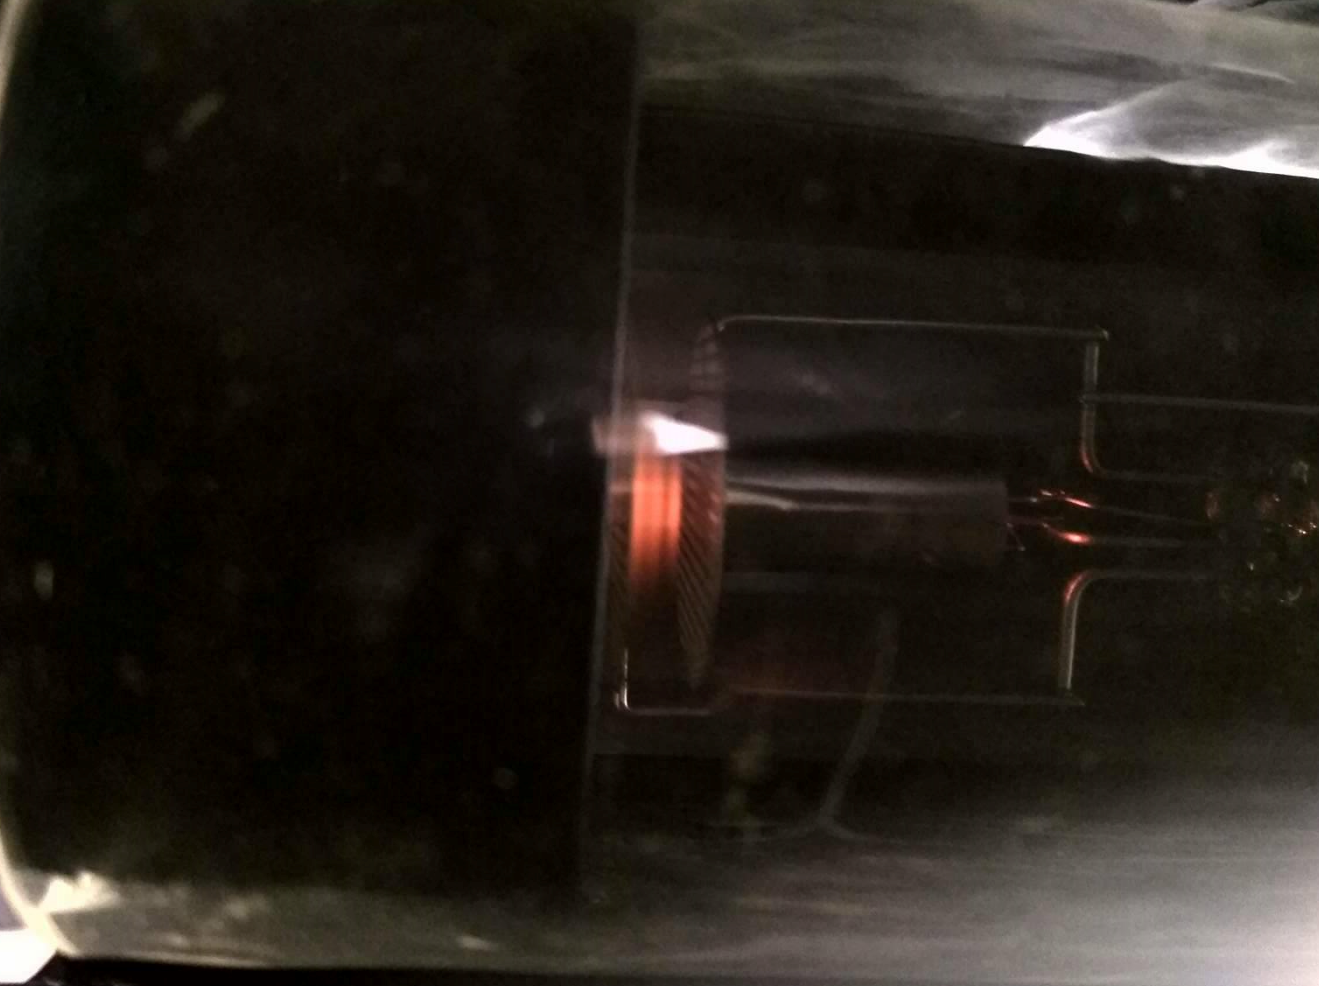
\includegraphics[scale=0.35]{fo1.png}
\end{figure}
\end{document}